\section{Caratteristiche dei materiali}
\diapo{Nanoparticelle: inorganiche o organiche?}
Le nanoparticelle vengono utilizzate come \alert{trasportatrici di elettroni}.\\
Pro e contro delle nanoparticelle inorganiche (\emph{quantum dots} semiconduttori) rispetto alle organiche (fullereni modificati o nanotubi):

\pause

 
\begin{itemize}
 \item[\checkmark] livelli energetici variabili con la dimensione,
 \item[\checkmark] coefficienti di assorbimento della luce più alti,
 \item[\checkmark] mobilità elettronica più alta,
 \item[$\times$] dimensioni maggiori dei fullereni perciò interfaccia minore,
 \item[$\times$] sono state ottenute efficienze minori a causa della \alert{aggregazione}.
\end{itemize}


\pause

 

Quest'ultimo problema si può limitare usando \\un \alert{polimero con gruppi leganti}.
\end{frame}

\diapo{Nanoparticelle inorganiche: quali? CdSe}
Molti semiconduttori inorganici si trovano in letteratura per nanoparticelle in celle ibride.
\begin{center}
  \begin{minipage}{7.5cm}   
\begin{block}{In questa tesi:} Sono state sintetizzate nanoparticelle di CdSe.\end{block}
\end{minipage}
\end{center}
\begin{itemize}
 \item efficienze energetiche più alte,
 \item anche in forme complesse.
\end{itemize}

\end{frame}

%%%%%%%%%%%%%%%%%%%%%%%%%%%%%%%%%%%%%%%%%%%%%%%%%%%%%%%%%%%%%%%%%%%%%%%%%%%%%%%%%%%%%%%%%%%%%%%%%%%%%%%%%%%%%%%%%%%%%%%%%%%%%%%%%%%%

\subsection{Polimeri coniugati: coniugazione e catene laterali}
\begin{frame}
\frametitle{Polimeri coniugati: coniugazione e catene laterali}
Il polimero coniugato assorbe la maggior parte della luce e \alert{trasporta le lacune}. \\

\pause

 

\begin{itemize}
\item Minore è la differenza HOMO - LUMO e maggiore è la porzione di spettro solare assorbito.
\item Questa differenza e la lunghezza di coniugazione dipendono dalla \alert{planarità} del polimero. 
\item Le catene laterali alifatiche aumentano la solubilità ma diminuiscono la planarità.
\end{itemize}\end{frame}

%%%%%%%%%%%%%%%%%%%%%%%%%%%%%%%%%%%%%%%%%%%%%%%%%%%%%%%%%%%%%%%%%%%%%%%%%%%%%%%%%%%%%%%%%%%%%%%%%%%%%%%%%%%%%%%%%%%%%%%%%%%%%%%%%%%%
{
\setbeamertemplate{navigation symbols}{}
\diapo{Polimeri coniugati: quale? Politiofene regioregolare}
\begin{center}
  \begin{minipage}{8.3cm}
\begin{block}{In questa tesi:}È stato sintetizzato poli(3-esiltiofene) regioregolare \\contenente un gruppo legante. \end{block}
\end{minipage}
\end{center}
Perché:
\begin{itemize}
\item livelli energetici adatti ad essere accoppiati con il CdSe, 
\item se regioregolare (vedi figura) si possono raggiungere lunghezze di coniugazione di 20 monomeri.
\end{itemize}
\begin{figure}{\centering{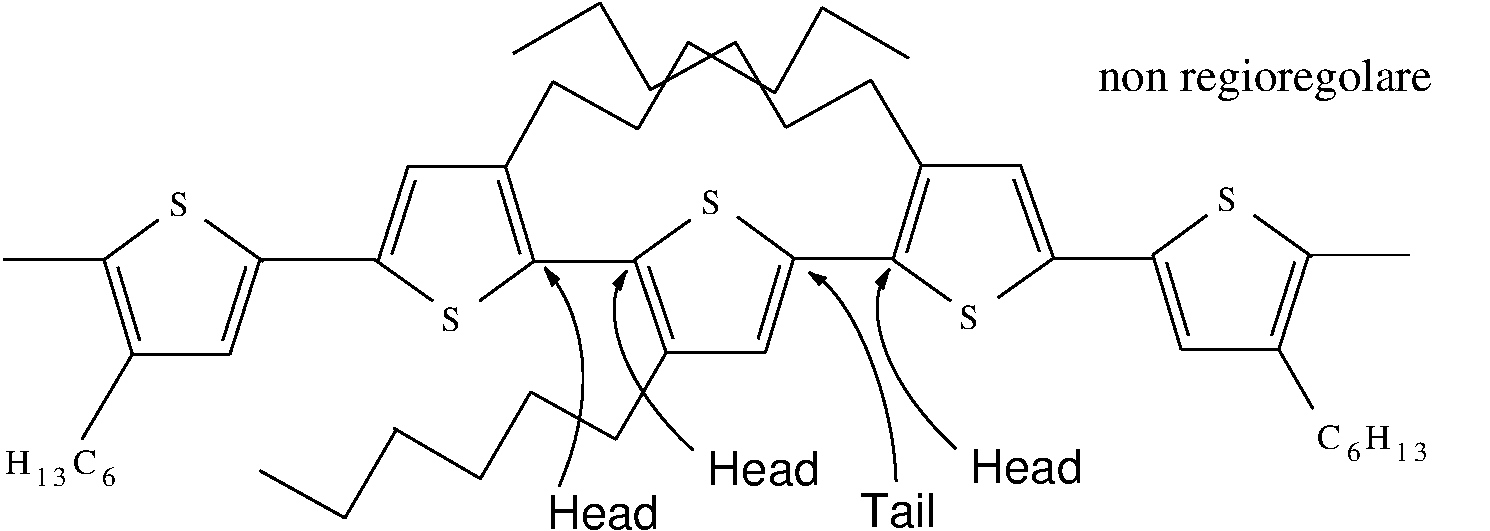
\includegraphics[width=0.67\textwidth]{Immagini_Tesi/p3ht-hhth3.pdf}}}\end{figure}
\end{frame}
}
%%%%%%%%%%%%%%%%%%%%%%%%%%%%%%%%%%%%%%%%%%%%%%%%%%%%%%%%%%%%%%%%%%%%%%%%%%%%%%%%%%%%%%%%%%%%%%%%%%%%%%%%%%%%%%%%%%%%%%%%%%%%%%%%%%%%








